
\documentclass[
    article, 
    12pt,				% tamanho da fonte
	oneside,			% para impressão apenas no recto. Oposto a twoside
	a4paper,			% tamanho do papel. 
	% -- opções da classe abntex2 --
	chapter=TITLE,		% títulos de capítulos convertidos em letras maiúsculas
	section=TITLE,		% títulos de seções convertidos em letras maiúsculas
	%subsection=TITLE,	% títulos de subseções convertidos em letras maiúsculas
	%subsubsection=TITLE % títulos de subsubseções convertidos em letras maiúsculas
	% -- opções do pacote babel --
	english,			% idioma adicional para hifenização
	english,				% o último idioma é o principal do documento
	sumario=tradicional
]{abntex2}

\usepackage[alf]{abntex2cite}
\usepackage{graphicx,url}
% \usepackage[USenglish,brazil]{babel}   
\usepackage[utf8]{inputenc}
\usepackage{lmodern}			% Usa a fonte Latin Modern
\usepackage[T1]{fontenc}		% Selecao de codigos de fonte.
\usepackage{indentfirst}		% Indenta o primeiro parágrafo de cada seção.
\usepackage{nomencl} 			% Lista de simbolos
\usepackage{color}				% Controle das cores
\usepackage{microtype} 			% para melhorias de justificação
\usepackage[english,hyperpageref]{backref}	 % Paginas com as citações na bibl
\usepackage{helvet}             % Fonte Helvica - Arial

\renewcommand{\familydefault}{\sfdefault}    % set the default font as serif, i.e., Arial
     
% ---
% compila o indice
% ---
\makeindex
% ---

% ---
% Altera as margens padrões
% ---
\setlrmarginsandblock{2.54cm}{2.54cm}{*}
\setulmarginsandblock{2.44cm}{2.54cm}{*}
\checkandfixthelayout
% ---

% --- 
% Espaçamentos entre linhas e parágrafos 
% --- 

% O tamanho do parágrafo é dado por:
\setlength{\parindent}{1cm}

% Controle do espaçamento entre um parágrafo e outro:
\setlength{\parskip}{0.2cm}  % tente também \onelineskip

% Espaçamento simples
\SingleSpacing

\renewcommand{\baselinestretch}{1.5} 


% Remove espaçamento do resumo
\setlength\absleftindent{0cm}
\setlength\absrightindent{0cm}
% Garante que a fonte do texto do abstract será a mesma do documento, pois
% na classe memoir está \small
\renewcommand{\abstracttextfont}{\normalfont\normalsize}

\setlength{\footmarkwidth}{1.8em}
\setlength{\footmarksep}{-\footmarkwidth}
\setlength{\footparindent}{1em}

% Define como negrito usando tamanho normal das fontes na seção e capítulo
\renewcommand{\ABNTEXchapterfont}{\bfseries}

% Define a subseção como negrito e tamanho normal
\renewcommand{\ABNTEXsubsectionfont}{\bfseries}
\renewcommand{\ABNTEXsubsectionfontsize}{\normalsize}

% Define a seção terciária como itálico e tamanho normal
\renewcommand{\ABNTEXsubsubsectionfont}{\itshape}
\renewcommand{\ABNTEXsubsubsectionfontsize}{\normalsize}

\renewcommand{\ABNTEXsectionfontsize}{\normalsize}
\renewcommand{\ABNTEXchapterfontsize}{\normalsize}

\date{September 22, 2021}

\renewcommand{\imprimirautor}{
  \begin{flushright}
   \theauthor
   \footnote{Student of the computer science course at La Salle University - Unilasalle, enrolled in the Artificial Intelligence course under the guidance of Prof. Filipe de Aguiar Geissler. E-mail: davi.201810357@unilasalle.edu.br. Date of submission: \thedate }
  \end{flushright}
}



\title{ \textbf{\uppercase{A review of AlphaStar multi-agent reinforcement learning}}}

\autor{
Davi F. Henrique
}

\begin{document} 

\selectlanguage{english}

\thetitle

\imprimirautor

\citeoption{ABNT-final}

\begin{resumo}
 There are many real-world problems that requires artificial agents to compete and cooperate with other agents to achieve a common goal. 
 In this paper, we reviewed the AlphaStar agent from the published paper \cite{vinyals_grandmaster_2019} by doing comparative analysis with other papers in the same field.
 
 \vspace{\onelineskip}
 Keywords: Deepmind, multiagent, reinforcement learning
\end{resumo}


\section{Introduction}

StarCraft II is a real-time online strategy game (RTS) where players can play with three different races. 
The game involves the balance of high level economic decisions (Macromanagement) with the control of hundreds of individual units. 
The game domain is complex, raising important challenges due to the space of the strategies and counter-strategies, having combinatorial actions that can be done. 
Considering that the gameplay has a duration of ten minutes, there are thousands of actions made in real-time.
Each action has a type with parameters such as who will execute it, where to target, among locations on the map or units nearby.

To approach those challenges, the authors of the AlphaStar paper \cite{vinyals_grandmaster_2019} used a general purpose learning method, a multiagent reinforcement learning. 
The algorithm uses data from both human and agent games, continually adapting its strategies throughout the games.

The agent has a rate limit in their actions and reaction time in the game, having network latency and computation time. 
Its actions per minute (APM) is limited as in the \autoref{fig:monitoring_layer}.  

\begin{figure}[ht]
    \centering
    \caption{Monitoring layer}
    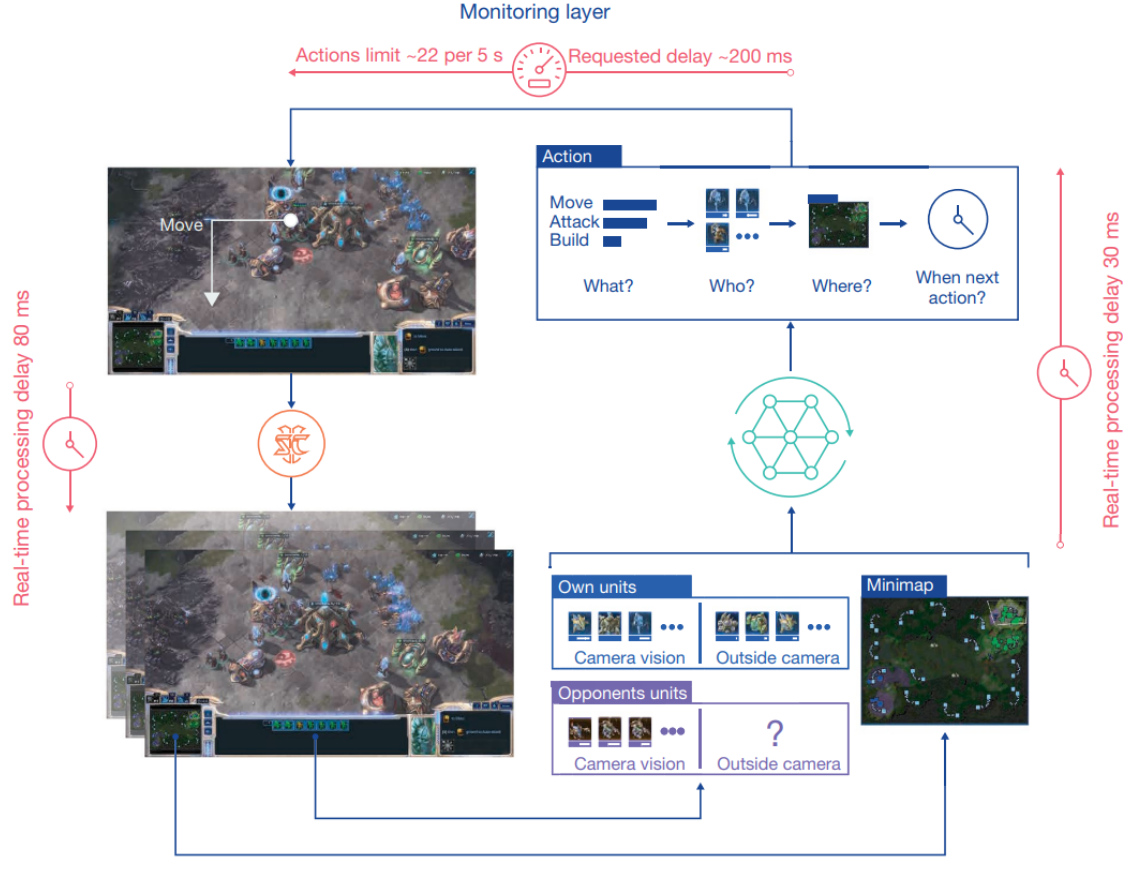
\includegraphics[width=\textwidth]{images/monitoring_layer.png}
    \fonte{\citeonline[p. 2]{vinyals_grandmaster_2019}}
    \label{fig:monitoring_layer}
\end{figure}

\section{The model}

AlphaStar has a neural network with parameters $\theta$ that represents a policy $\pi(a_t | s_t,z) = P[a_t | s_t,z]$. 
This network receives all observations from the game as inputs and selects actions as output. 
The agent's architecture consists of general purpose neural networks components such as long short-term memory (LSTM) system, for temporal sequence of partial observations and a recurrent point network.

The league consists of three distinct types of agent, having the main differences in their mechanism for selecting the opponent mixture.
The main agent use a prioritized fictitious self-play (PFSP) mechanism, which adapts the mixture probabilities proportionally to the win rate of each opponent. 
The exploiter agents have the main objective of identify potential exploits in the main agents. 
The league exploiter agents have the goal of finding systemic weaknesses in the entire league.

\section{Training setup}

The agent parameters were initially trained by supervised learning, using a public available dataset of humans playing the game. 
The optimizer used in supervised learning was Kullback-Leibler (KL) divergence between its output and the human actions replay.
The policy was trained to predict each action.

Subsequently, the pool of agents are trained with reinforcement learning using the human data and their experience, to update their policy combined with the optimizer. 
During the training phase, the agents make copies of themselves and train against all of them, as shown in the \autoref{fig:trainig_setup}c. 
With the objective of improve its response to maximize the win rate against a mixture of opponents.
The \autoref{fig:trainig_setup}b illustrates the training flow. 


\begin{figure}[ht]
    \centering
    \caption{Training Setup}
    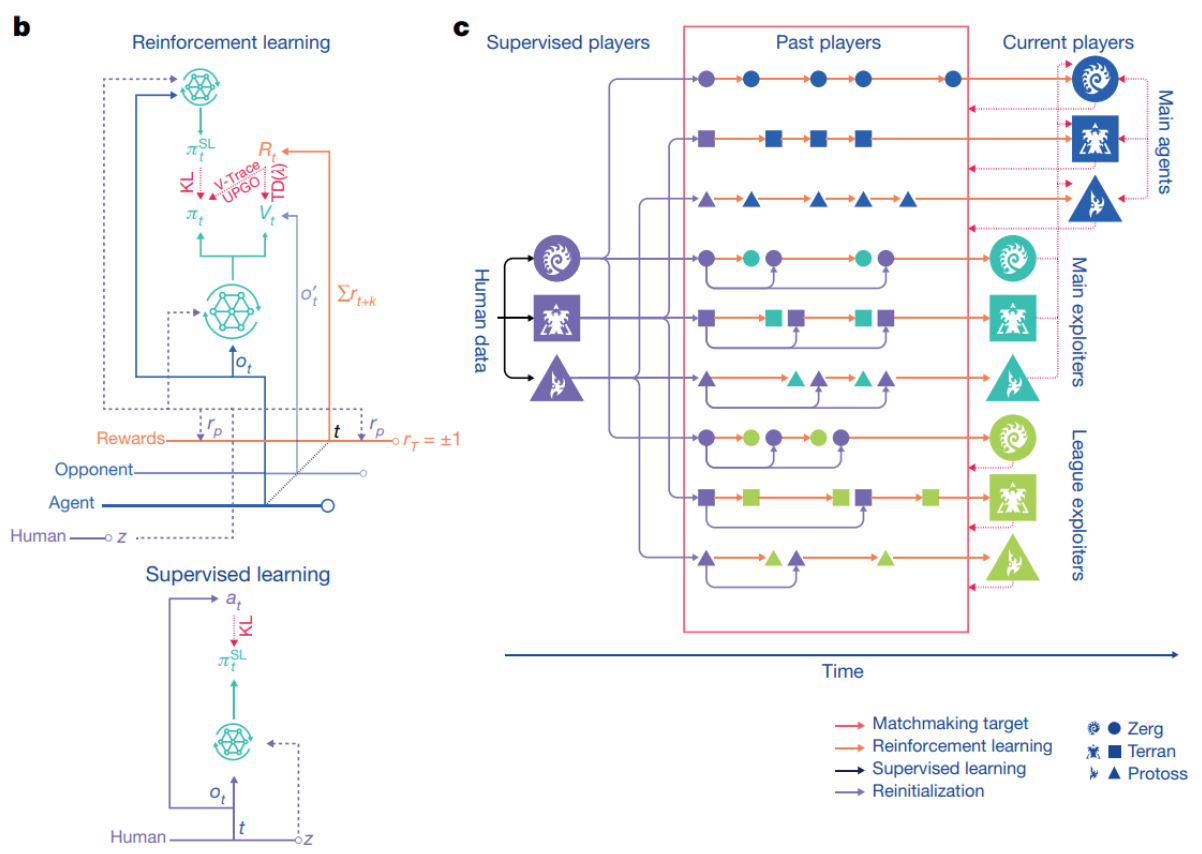
\includegraphics[width=\textwidth]{images/training.png}
    \fonte{\citeonline[p. 2]{vinyals_grandmaster_2019}}
    \label{fig:trainig_setup}
\end{figure}


\section{AlphaStar results}

The AlphaStar Supervised and Mid started from an unranked rating on Battle.net and played 30 and 60 games, respectively, for each race.
The AlphaStar Final was evaluated from AlphaStar Mid's rating for more 30 games in each race.

AlphaStar Final achieved Grandmaster level in all three races, being above 99.8\% of ranked human players.
The Match Making Rating (MMR) achieved was 6,275 for Protoss, 6,048 for Terran and 5,835 for Zerg.
The AlphaStar Supervised had an average rating of 3,699 MMR, which is above 84\% of StarCraft II players (\autoref{fig:alphaStar_results}a).

\begin{figure}[ht]
    \centering
    \caption{AlphaStar results}
    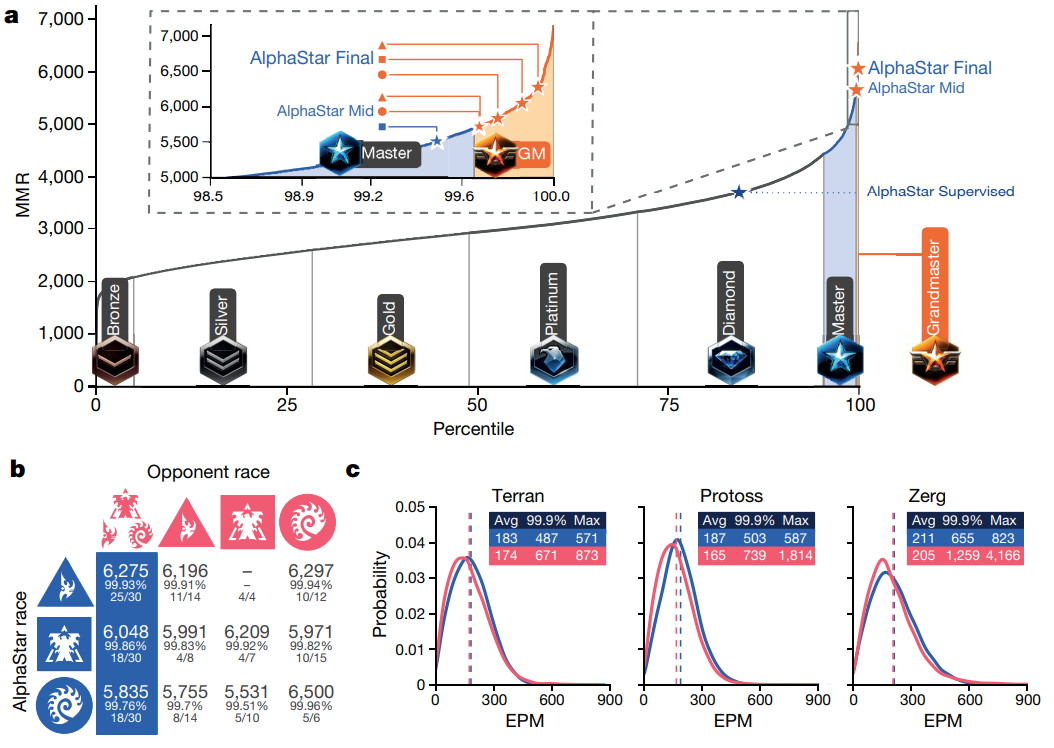
\includegraphics[width=\textwidth]{images/results.png}
    \fonte{\citeonline[p. 3]{vinyals_grandmaster_2019}}
    \label{fig:alphaStar_results}
\end{figure}


\section{Considerations}

The overall results and the strategies used by AlphaStar shows the good performance of the agents. 
The matches recorded demonstrate the strategies not expected to be done by common players, but used by AlphaStar throughout the games.
Such as strange unit composition, some plays that are considered very poor, however the agent wins in the end.

AlphaStar neural network uses a total of 139 million parameters, which is much bigger than TStarBot-X, a proposed agent with similar action space which uses only 20 million parameters \cite{han_tstarbotx_2021}.
Both agents started learning by imitating human players in a supervised manner, which has been demonstrated as an effective way to provide an agent a good initial policy.


\bibliography{./references/abnt-template}

\end{document}
